% !TEX program = pdflatex
\documentclass[aspectratio=169, 11pt]{beamer}

% ── Theme & Colors ──
\usetheme{Madrid}
\usecolortheme{whale}
\definecolor{deepblue}{RGB}{0, 51, 102}
\definecolor{accentred}{RGB}{180, 30, 30}
\definecolor{softgreen}{RGB}{34, 139, 34}
\definecolor{lightgray}{RGB}{240, 240, 240}
\definecolor{hlrow}{RGB}{220, 235, 255}
\definecolor{amber}{RGB}{255, 165, 0}

\setbeamercolor{frametitle}{bg=deepblue, fg=white}
\setbeamercolor{title}{bg=deepblue, fg=white}
\setbeamercolor{block title}{bg=deepblue, fg=white}
\setbeamercolor{block body}{bg=lightgray, fg=black}
\setbeamercolor{block title alerted}{bg=accentred, fg=white}
\setbeamercolor{block body alerted}{bg=lightgray, fg=black}
\setbeamercolor{block title example}{bg=softgreen, fg=white}
\setbeamercolor{block body example}{bg=lightgray, fg=black}
\setbeamercolor{item}{fg=deepblue}
\setbeamertemplate{navigation symbols}{}
\setbeamertemplate{footline}[frame number]

% ── Packages ──
\usepackage{amsmath, amssymb, mathtools}
\usepackage{booktabs}
\usepackage{array}
\usepackage{tikz}
\usetikzlibrary{arrows.meta, positioning, shapes.geometric, calc, decorations.pathmorphing, fit, backgrounds}
\usepackage{pgfplots}
\pgfplotsset{compat=1.18}
\usepackage{colortbl}
\usepackage{multirow}
\usepackage{graphicx}
\usepackage{hyperref}
\usepackage{adjustbox}
\usepackage{tabularx}
\usepackage{xcolor}
\usepackage{pifont}
\usepackage{algorithm}
\usepackage{algorithmic}

\newcommand{\cmark}{\textcolor{softgreen}{\ding{51}}}
\newcommand{\xmark}{\textcolor{accentred}{\ding{55}}}

% ── Title Page ──
\title[VFL Unlearning Framework]{Vertical Federated Unlearning:\\A Comprehensive Framework with Entanglement Analysis}
\subtitle{Knowledge Distillation, Gradient Ascent \& Jacobian-Based Diagnostics}
\author{VFU-ML Project}
\date{\today}
\institute{CSE 472 --- Machine Learning}

\begin{document}

% ================================================================
%  TITLE
% ================================================================
\begin{frame}
  \titlepage
\end{frame}

% ================================================================
%  OUTLINE
% ================================================================
\begin{frame}{Outline}
  \tableofcontents
\end{frame}

% ================================================================
\section{Problem Statement}
% ================================================================

\begin{frame}{Problem Statement}
  \begin{columns}[T]
    \begin{column}{0.55\textwidth}
      \begin{alertblock}{The Challenge}
        In \textbf{Vertical Federated Learning (VFL)}, multiple parties collaboratively train a model by contributing \emph{different features} of the same samples. Data privacy regulations (GDPR, CCPA) mandate the \textbf{``Right to be Forgotten''}.
      \end{alertblock}
      \vspace{0.3cm}
      \textbf{Three unlearning scenarios:}
      \begin{enumerate}
        \item A \textbf{passive party} wants to leave the federation
        \item A party wants to remove \textbf{specific features}
        \item The active party must forget \textbf{specific samples}
      \end{enumerate}
    \end{column}
    \begin{column}{0.42\textwidth}
      \begin{center}
        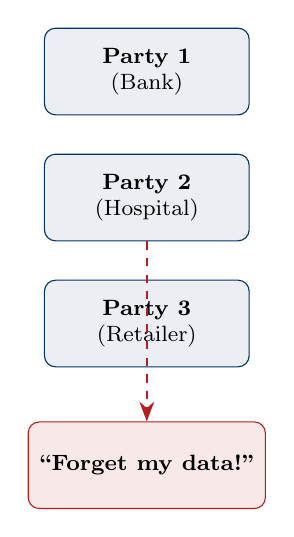
\begin{tikzpicture}[
          box/.style={rectangle, draw=deepblue, fill=deepblue!8, rounded corners=4pt,
                      minimum width=2.6cm, minimum height=1.1cm, align=center, font=\footnotesize},
          warn/.style={rectangle, draw=accentred, fill=accentred!10, rounded corners=4pt,
                       minimum width=2.8cm, minimum height=1.1cm, align=center, font=\footnotesize},
          arr/.style={-{Stealth[length=2.5mm]}, thick, deepblue}
        ]
          \node[box] (p1) at (0,2.2) {\textbf{Party 1}\\(Bank)};
          \node[box] (p2) at (0,0.6) {\textbf{Party 2}\\(Hospital)};
          \node[box] (p3) at (0,-1.0) {\textbf{Party 3}\\(Retailer)};
          \node[warn] (q) at (0,-2.8) {\textbf{``Forget my data!''}};
          \draw[-{Stealth[length=2.5mm]}, thick, accentred, dashed] (p2) -- (q);
        \end{tikzpicture}
      \end{center}
    \end{column}
  \end{columns}
\end{frame}

\begin{frame}{Why Is VFL Unlearning Harder Than Centralized?}
  \begin{center}
    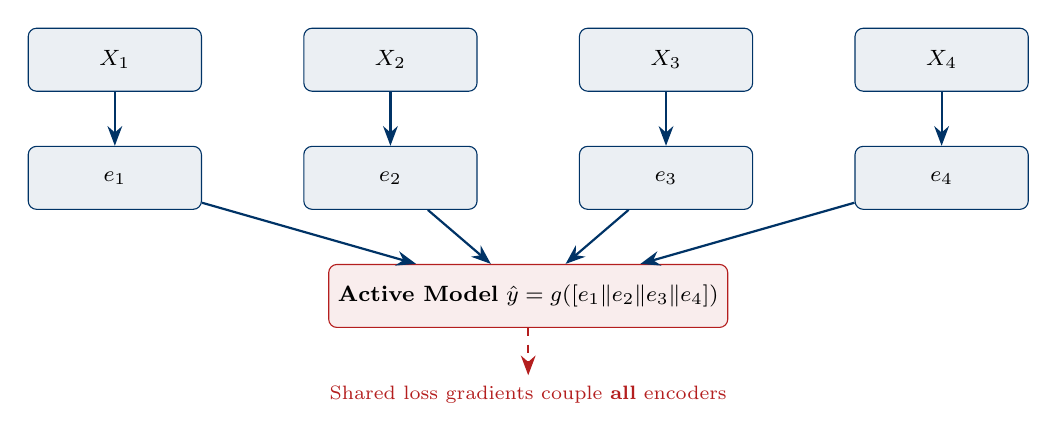
\begin{tikzpicture}[
      box/.style={rectangle, draw=deepblue, fill=deepblue!8, rounded corners=3pt,
                  minimum width=2.2cm, minimum height=0.8cm, align=center, font=\footnotesize},
      arr/.style={-{Stealth[length=2.5mm]}, thick, deepblue}
    ]
      \node[box] (x1) at (0,2.5) {$X_1$};
      \node[box] (x2) at (3.5,2.5) {$X_2$};
      \node[box] (x3) at (7,2.5) {$X_3$};
      \node[box] (x4) at (10.5,2.5) {$X_4$};

      \node[box] (e1) at (0,1.0) {$e_1$};
      \node[box] (e2) at (3.5,1.0) {$e_2$};
      \node[box] (e3) at (7,1.0) {$e_3$};
      \node[box] (e4) at (10.5,1.0) {$e_4$};

      \draw[arr] (x1)--(e1); \draw[arr] (x2)--(e2);
      \draw[arr] (x3)--(e3); \draw[arr] (x4)--(e4);

      \node[box, draw=accentred, fill=accentred!8, minimum width=4cm] (top) at (5.25,-0.5) {\textbf{Active Model} $\hat{y} = g([e_1\|e_2\|e_3\|e_4])$};
      \draw[arr] (e1)--(top); \draw[arr] (e2)--(top);
      \draw[arr] (e3)--(top); \draw[arr] (e4)--(top);

      \draw[-{Stealth[length=2.5mm]}, thick, accentred, dashed] (top.south) -- ++(0,-0.6)
        node[below, font=\scriptsize, text=accentred] {Shared loss gradients couple \textbf{all} encoders};
    \end{tikzpicture}
  \end{center}
  \vspace{0.3cm}
  \begin{alertblock}{Key Difficulty}
    \begin{itemize}
      \item Retraining from scratch is \textbf{prohibitively expensive} (communication rounds)
      \item Naive removal causes \textbf{cascading accuracy drops} across remaining parties
      \item No raw data sharing $\Rightarrow$ unlearning must work with \textbf{embeddings only}
    \end{itemize}
  \end{alertblock}
\end{frame}

% ================================================================
\section{Solution Architecture}
% ================================================================

\begin{frame}{VFL Split Learning Architecture}
  \begin{center}
    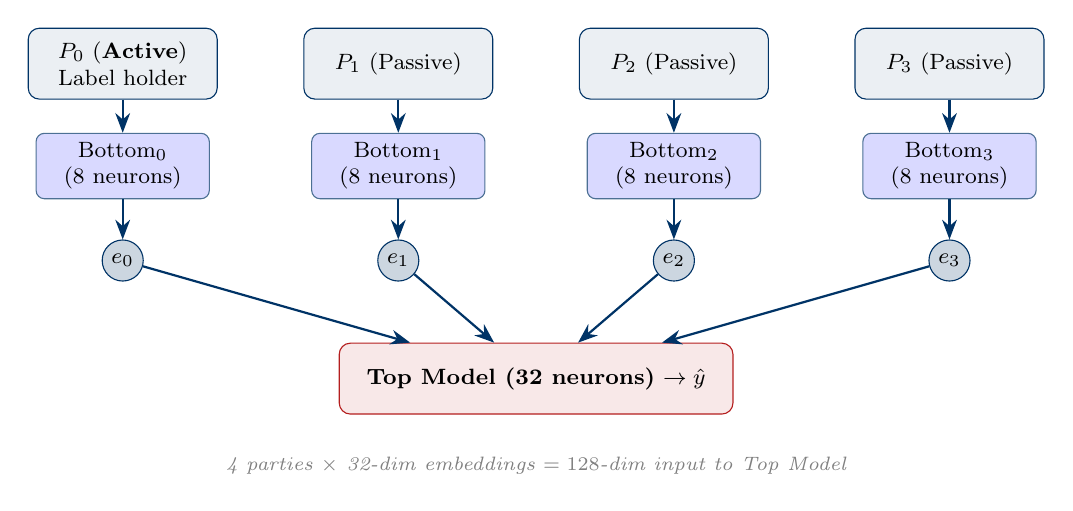
\begin{tikzpicture}[
      party/.style={rectangle, draw=deepblue, fill=deepblue!8, rounded corners=4pt,
                    minimum width=2.4cm, minimum height=0.9cm, align=center, font=\footnotesize},
      enc/.style={rectangle, draw=deepblue!70, fill=blue!15, rounded corners=3pt,
                  minimum width=2.2cm, minimum height=0.7cm, align=center, font=\footnotesize},
      emb/.style={circle, draw=deepblue, fill=deepblue!20, inner sep=2pt, font=\footnotesize},
      active/.style={rectangle, draw=accentred, fill=accentred!10, rounded corners=4pt,
                     minimum width=3.0cm, minimum height=0.9cm, align=center, font=\footnotesize},
      arr/.style={-{Stealth[length=2.5mm]}, thick, deepblue}
    ]
      \node[party]  (p0) at (0,   2.8) {$P_0$ (\textbf{Active})\\Label holder};
      \node[party]  (p1) at (3.5, 2.8) {$P_1$ (Passive)};
      \node[party]  (p2) at (7.0, 2.8) {$P_2$ (Passive)};
      \node[party]  (p3) at (10.5,2.8) {$P_3$ (Passive)};

      \node[enc] (e0) at (0,   1.5) {Bottom$_0$\\(8 neurons)};
      \node[enc] (e1) at (3.5, 1.5) {Bottom$_1$\\(8 neurons)};
      \node[enc] (e2) at (7.0, 1.5) {Bottom$_2$\\(8 neurons)};
      \node[enc] (e3) at (10.5,1.5) {Bottom$_3$\\(8 neurons)};

      \draw[arr] (p0)--(e0); \draw[arr] (p1)--(e1);
      \draw[arr] (p2)--(e2); \draw[arr] (p3)--(e3);

      \node[emb] (em0) at (0,   0.3) {$e_0$};
      \node[emb] (em1) at (3.5, 0.3) {$e_1$};
      \node[emb] (em2) at (7.0, 0.3) {$e_2$};
      \node[emb] (em3) at (10.5,0.3) {$e_3$};

      \draw[arr] (e0)--(em0); \draw[arr] (e1)--(em1);
      \draw[arr] (e2)--(em2); \draw[arr] (e3)--(em3);

      \node[active, minimum width=5cm] (top) at (5.25, -1.2) {\textbf{Top Model (32 neurons)} $\to \hat{y}$};
      \draw[arr] (em0)--(top); \draw[arr] (em1)--(top);
      \draw[arr] (em2)--(top); \draw[arr] (em3)--(top);

      \node[font=\scriptsize\itshape, text=gray] at (5.25, -2.3) {4 parties $\times$ 32-dim embeddings $= 128$-dim input to Top Model};
    \end{tikzpicture}
  \end{center}
\end{frame}

\begin{frame}{Proposed Framework: Seven Algorithms}
  \begin{center}
    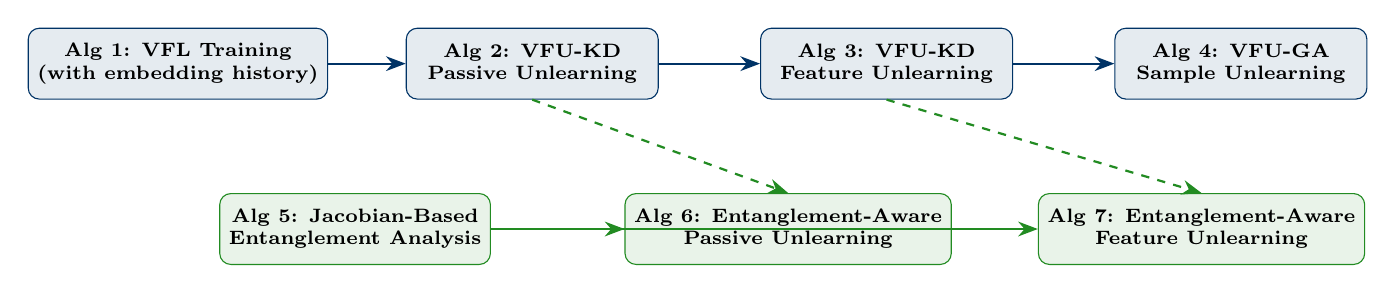
\begin{tikzpicture}[
      alg/.style={rectangle, draw=deepblue, fill=deepblue!10, rounded corners=4pt,
                  minimum width=3.2cm, minimum height=0.9cm, align=center, font=\scriptsize\bfseries},
      ealg/.style={rectangle, draw=softgreen, fill=softgreen!10, rounded corners=4pt,
                   minimum width=3.2cm, minimum height=0.9cm, align=center, font=\scriptsize\bfseries},
      arr/.style={-{Stealth[length=2.5mm]}, thick, deepblue}
    ]
      \node[alg]  (a1) at (0,   2.4) {Alg 1: VFL Training\\(with embedding history)};
      \node[alg]  (a2) at (4.5, 2.4) {Alg 2: VFU-KD\\Passive Unlearning};
      \node[alg]  (a3) at (9.0, 2.4) {Alg 3: VFU-KD\\Feature Unlearning};
      \node[alg]  (a4) at (13.5,2.4) {Alg 4: VFU-GA\\Sample Unlearning};

      \node[ealg] (a5) at (2.25, 0.3) {Alg 5: Jacobian-Based\\Entanglement Analysis};
      \node[ealg] (a6) at (7.75, 0.3) {Alg 6: Entanglement-Aware\\Passive Unlearning};
      \node[ealg] (a7) at (13.0,0.3) {Alg 7: Entanglement-Aware\\Feature Unlearning};

      \draw[arr] (a1)--(a2); \draw[arr] (a2)--(a3); \draw[arr] (a3)--(a4);
      \draw[-{Stealth[length=2.5mm]}, thick, softgreen] (a5)--(a6);
      \draw[-{Stealth[length=2.5mm]}, thick, softgreen] (a5)--(a7);
      \draw[-{Stealth[length=2.5mm]}, thick, softgreen, dashed] (a2.south) -- (a6.north);
      \draw[-{Stealth[length=2.5mm]}, thick, softgreen, dashed] (a3.south) -- (a7.north);
    \end{tikzpicture}
  \end{center}
  \vspace{0.2cm}
  \begin{columns}[T]
    \begin{column}{0.48\textwidth}
      \begin{block}{Core Unlearning (Alg 1--4)}
        \begin{itemize}
          \item \textbf{VFU-KD}: Knowledge Distillation to unlearn parties/features
          \item \textbf{VFU-GA}: Gradient Ascent for sample forgetting
        \end{itemize}
      \end{block}
    \end{column}
    \begin{column}{0.48\textwidth}
      \begin{exampleblock}{Entanglement-Aware (Alg 5--7)}
        \begin{itemize}
          \item \textbf{Diagnosis}: Jacobian SVD $\rho$ metric
          \item \textbf{Mitigation}: Conditional retraining of at-risk parties
        \end{itemize}
      \end{exampleblock}
    \end{column}
  \end{columns}
\end{frame}

% ================================================================
\section{Dataset Definition}
% ================================================================

\begin{frame}{Datasets}
  \begin{columns}[T]
    \begin{column}{0.48\textwidth}
      \begin{block}{UCI Adult (Census Income)}
        \begin{itemize}
          \item \textbf{Samples:} 32,561
          \item \textbf{Features:} 14 (mixed categorical/numerical)
          \item \textbf{Task:} Binary --- income $>$\$50K
          \item \textbf{Split:} 80/20 train/test
          \item \textbf{Class dist:} $\{0: 24720, 1: 7841\}$
        \end{itemize}
      \end{block}
    \end{column}
    \begin{column}{0.48\textwidth}
      \begin{block}{German Credit}
        \begin{itemize}
          \item \textbf{Samples:} 1,000
          \item \textbf{Features:} 20 (mixed)
          \item \textbf{Task:} Binary --- credit risk
          \item \textbf{Split:} 80/20 train/test
          \item \textbf{Class dist:} $\{1: 700, 0: 300\}$
        \end{itemize}
      \end{block}
    \end{column}
  \end{columns}

  \vspace{0.4cm}
  \begin{block}{Vertical Partitioning (4 Parties)}
    Features are \textbf{equally partitioned} across 4 parties using \texttt{VFLDataPartitioner}:
    \begin{itemize}
      \item \textbf{Party 0} (Active): holds labels + its feature subset
      \item \textbf{Parties 1--3} (Passive): hold disjoint feature subsets, no labels
    \end{itemize}
  \end{block}
\end{frame}

% ================================================================
\section{Solution Mechanism}
% ================================================================

% ── Algorithm 1: VFL Training ──
\begin{frame}{Algorithm 1: VFL Training with Embedding History}
  \begin{columns}[T]
    \begin{column}{0.50\textwidth}
      \begin{block}{Pseudocode}
        \begin{algorithmic}[1]
          \footnotesize
          \STATE \textbf{Input:} Passive parties $P_1,\ldots,P_k$; Active $P_a$; $\eta_1, \eta_2$
          \FOR{epoch $t = 1, \ldots, T$}
            \STATE Sample minibatch $\mathcal{D}$
            \FOR{each party $P_i$ \textbf{in parallel}}
              \STATE $e_i \gets G(\theta_i, \mathcal{D})$
              \STATE Send $e_i$ to $P_a$
            \ENDFOR
            \STATE Concatenate $[e_1, \ldots, e_k]$
            \STATE \textbf{Store} $E_i^t \gets e_i$ \hfill $\triangleright$ \textit{for unlearning}
            \STATE $\hat{y} = f(\theta_a, [e_1,\ldots,e_k])$
            \STATE $\mathcal{L} = \ell(\hat{y}, y)$
            \STATE $\theta_a \gets \theta_a - \eta_1 \nabla_{\theta_a} \mathcal{L}$
            \STATE Send $\partial\mathcal{L}/\partial e_i$ to each $P_i$
            \STATE $\theta_i \gets \theta_i - \eta_2 \nabla_{\theta_i} \mathcal{L}$
          \ENDFOR
        \end{algorithmic}
      \end{block}
    \end{column}
    \begin{column}{0.47\textwidth}
      \begin{center}
        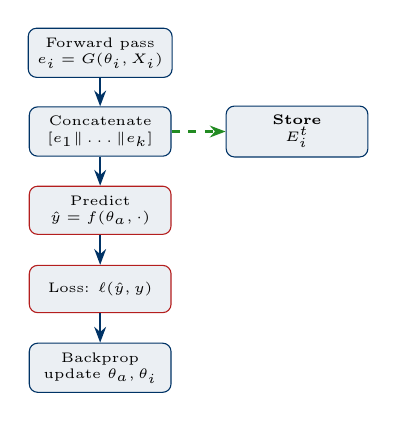
\begin{tikzpicture}[
          box/.style={rectangle, draw=deepblue, fill=deepblue!8, rounded corners=3pt,
                      minimum width=1.8cm, minimum height=0.6cm, align=center, font=\tiny},
          arr/.style={-{Stealth[length=2mm]}, thick, deepblue}
        ]
          \node[box] (fwd) at (0,3.0) {Forward pass\\$e_i = G(\theta_i, X_i)$};
          \node[box] (cat) at (0,2.0) {Concatenate\\$[e_1\|\ldots\|e_k]$};
          \node[box] (store) at (2.5,2.0) {\textbf{Store}\\$E_i^t$};
          \node[box, draw=accentred] (pred) at (0,1.0) {Predict\\$\hat{y} = f(\theta_a, \cdot)$};
          \node[box, draw=accentred] (loss) at (0,0) {Loss: $\ell(\hat{y}, y)$};
          \node[box] (back) at (0,-1.0) {Backprop\\update $\theta_a, \theta_i$};

          \draw[arr] (fwd)--(cat); \draw[arr] (cat)--(pred);
          \draw[arr] (pred)--(loss); \draw[arr] (loss)--(back);
          \draw[arr, dashed, softgreen] (cat)--(store);
        \end{tikzpicture}
      \end{center}
      \vspace{0.2cm}
      \footnotesize
      \textbf{Hyperparameters:}\\
      $\eta_1 = \eta_2 = 0.01$, Batch $= 512$\\
      Optimizer: RAdam, Epochs: 50\\
      Embedding dim: 32
    \end{column}
  \end{columns}
\end{frame}

% ── Algorithm 2: VFU-KD Passive Unlearning ──
\begin{frame}{Algorithm 2: VFU-KD --- Passive Party Unlearning}
  \begin{columns}[T]
    \begin{column}{0.50\textwidth}
      \begin{block}{Pseudocode}
        \begin{algorithmic}[1]
          \footnotesize
          \STATE \textbf{Input:} Party $P_u$ to unlearn; historical $E_i^t$; $\eta_1$; $\lambda$
          \STATE Initialize student top model $\theta_a'$ (reduced input)
          \STATE Set original $\theta_a$ as \textbf{teacher} (frozen)
          \FOR{epoch $e = 1, \ldots, E$}
            \STATE $\hat{y}_S = f(\theta_a', [e_i]_{i \neq u})$ \hfill $\triangleright$ \textit{exclude $P_u$}
            \STATE $\hat{y}_T = f(\theta_a, [e_1,\ldots,e_k])$ \hfill $\triangleright$ \textit{all parties}
            \STATE $\mathcal{L} = (1-\lambda)\cdot\ell(\hat{y}_S, y) + \lambda\cdot\text{KL}(\hat{y}_S \| \hat{y}_T)$
            \STATE $\theta_a' \gets \theta_a' - \eta_1 \nabla_{\theta_a'} \mathcal{L}$
          \ENDFOR
          \RETURN $\theta_a'$
        \end{algorithmic}
      \end{block}
    \end{column}
    \begin{column}{0.47\textwidth}
      \begin{center}
        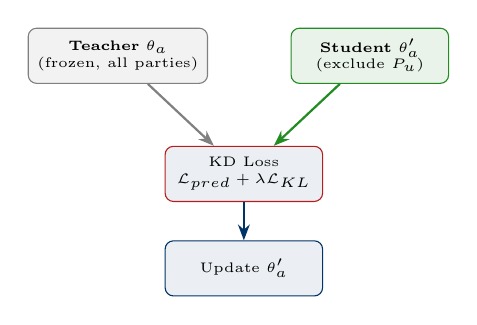
\begin{tikzpicture}[
          box/.style={rectangle, draw=deepblue, fill=deepblue!8, rounded corners=3pt,
                      minimum width=2cm, minimum height=0.7cm, align=center, font=\tiny},
          arr/.style={-{Stealth[length=2mm]}, thick, deepblue}
        ]
          \node[box, draw=gray, fill=gray!10] (teacher) at (-0.8,2.5) {\textbf{Teacher} $\theta_a$\\(frozen, all parties)};
          \node[box, draw=softgreen, fill=softgreen!10] (student) at (2.4,2.5) {\textbf{Student} $\theta_a'$\\(exclude $P_u$)};
          \node[box, draw=accentred] (kd) at (0.8,1.0) {KD Loss\\$\mathcal{L}_{pred} + \lambda \mathcal{L}_{KL}$};
          \node[box] (update) at (0.8, -0.2) {Update $\theta_a'$};

          \draw[arr, gray] (teacher)--(kd);
          \draw[arr, softgreen] (student)--(kd);
          \draw[arr] (kd)--(update);
        \end{tikzpicture}
      \end{center}
      \vspace{0.2cm}
      \footnotesize
      \textbf{Key idea:} Student learns to approximate teacher's output \emph{without} $P_u$'s embeddings.\\[0.2cm]
      $\lambda = 0.3$, $\eta_1 = 0.01$, 30 epochs
    \end{column}
  \end{columns}
\end{frame}

% ── Algorithm 3: VFU-KD Feature Unlearning ──
\begin{frame}{Algorithm 3: VFU-KD --- Feature Unlearning (Passive Side)}
  \begin{columns}[T]
    \begin{column}{0.50\textwidth}
      \begin{block}{Pseudocode}
        \begin{algorithmic}[1]
          \footnotesize
          \STATE \textbf{Input:} Party $P_u$; features $F_u$ to forget; $\eta_2$
          \STATE Init student $\theta_u'$ with $|\text{features}| - |F_u|$ inputs
          \STATE Set old $\theta_u$ as teacher (frozen)
          \FOR{epoch $e = 1, \ldots, E$}
            \STATE $e_T = G(\theta_u, D_{\text{full}})$ \hfill $\triangleright$ \textit{all features}
            \STATE $e_S = G(\theta_u', D_{\text{reduced}})$ \hfill $\triangleright$ \textit{sans $F_u$}
            \STATE $\mathcal{L} = \text{KL}(e_S \| e_T)$
            \STATE $\theta_u' \gets \theta_u' - \eta_2 \nabla \mathcal{L}$
          \ENDFOR
          \RETURN $\theta_u'$
        \end{algorithmic}
      \end{block}
      \vspace{0.2cm}
      \footnotesize
      \textbf{No communication needed} --- teacher \& student run locally at the passive party.
    \end{column}
    \begin{column}{0.47\textwidth}
      \begin{center}
        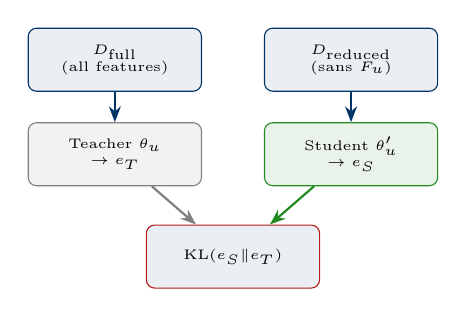
\begin{tikzpicture}[
          box/.style={rectangle, draw=deepblue, fill=deepblue!8, rounded corners=3pt,
                      minimum width=2.2cm, minimum height=0.8cm, align=center, font=\tiny},
          arr/.style={-{Stealth[length=2mm]}, thick, deepblue}
        ]
          \node[box] (full) at (0,3) {$D_{\text{full}}$\\(all features)};
          \node[box] (red) at (3,3) {$D_{\text{reduced}}$\\(sans $F_u$)};
          \node[box, draw=gray, fill=gray!10] (teach) at (0,1.8) {Teacher $\theta_u$\\$\to e_T$};
          \node[box, draw=softgreen, fill=softgreen!10] (stud) at (3,1.8) {Student $\theta_u'$\\$\to e_S$};
          \node[box, draw=accentred] (kl) at (1.5,0.5) {$\text{KL}(e_S \| e_T)$};

          \draw[arr] (full)--(teach); \draw[arr] (red)--(stud);
          \draw[arr, gray] (teach)--(kl); \draw[arr, softgreen] (stud)--(kl);
        \end{tikzpicture}
      \end{center}
      \vspace{0.2cm}
      \footnotesize
      $\eta_2 = 0.01$, 30 epochs, batch 512\\
      Student input dim = original $-$ $|F_u|$
    \end{column}
  \end{columns}
\end{frame}

% ── Algorithm 4: VFU-GA Sample Unlearning ──
\begin{frame}{Algorithm 4: VFU-GA --- Sample Unlearning}
  \begin{columns}[T]
    \begin{column}{0.50\textwidth}
      \begin{block}{Pseudocode}
        \begin{algorithmic}[1]
          \footnotesize
          \STATE \textbf{Input:} Forget set $B_u$; $\theta_a$; $\eta_1$; $\alpha$; epochs $E_u$
          \STATE Retrieve stored embeddings $E[B_u]$
          \FOR{epoch $e = 1, \ldots, E_u$}
            \STATE $E_{\text{forget}} \gets$ embeddings for $B_u$
            \STATE $E_{\text{retain}} \gets$ all other embeddings
            \STATE $\hat{y}_f = f(\theta_a, E_{\text{forget}})$;\quad $\hat{y}_r = f(\theta_a, E_{\text{retain}})$
            \STATE $\mathcal{L}_f = \ell(\hat{y}_f, y_f)$;\quad $\mathcal{L}_r = \ell(\hat{y}_r, y_r)$
            \STATE $\theta_a \gets \theta_a \underbrace{- \eta_1 \nabla\mathcal{L}_r}_{\text{retain}} \underbrace{+ \alpha \nabla\mathcal{L}_f}_{\text{forget}}$
          \ENDFOR
          \RETURN $\theta_a$
        \end{algorithmic}
      \end{block}
    \end{column}
    \begin{column}{0.47\textwidth}
      \begin{center}
        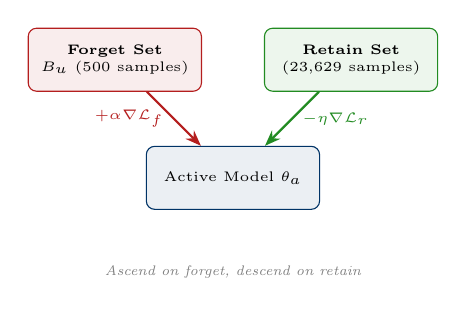
\begin{tikzpicture}[
          box/.style={rectangle, draw=deepblue, fill=deepblue!8, rounded corners=3pt,
                      minimum width=2.2cm, minimum height=0.8cm, align=center, font=\tiny},
          arr/.style={-{Stealth[length=2mm]}, thick}
        ]
          \node[box, draw=accentred, fill=accentred!8] (forget) at (0,2.5) {\textbf{Forget Set}\\$B_u$ (500 samples)};
          \node[box, draw=softgreen, fill=softgreen!8] (retain) at (3,2.5) {\textbf{Retain Set}\\(23,629 samples)};
          \node[box] (model) at (1.5,1.0) {Active Model $\theta_a$};

          \draw[arr, accentred] (forget) -- (model) node[midway, left, font=\tiny, text=accentred] {$+\alpha\nabla\mathcal{L}_f$};
          \draw[arr, softgreen] (retain) -- (model) node[midway, right, font=\tiny, text=softgreen] {$-\eta\nabla\mathcal{L}_r$};

          \node[font=\tiny\itshape, text=gray] at (1.5, -0.2) {Ascend on forget, descend on retain};
        \end{tikzpicture}
      \end{center}
      \vspace{0.2cm}
      \footnotesize
      $\eta_1 = 0.01$, $\alpha = 0.1$\\
      5 unlearning epochs\\
      \textbf{Key:} ``$+$'' on $\mathcal{L}_f$ = gradient \textbf{ascent} (forgetting)
    \end{column}
  \end{columns}
\end{frame}

% ── Algorithm 5: Feature Entanglement Analysis ──
\begin{frame}{Algorithm 5: Feature Entanglement Analysis}
  \begin{block}{Core Idea}
    Before unlearning, diagnose \textbf{cross-party coupling} via the mixed Hessian (Jacobian of gradient signals):
    \[
    J[d, f] = \mathbb{E}\!\left[\frac{\partial^2 \hat{y}}{\partial e_j[d] \cdot \partial X_k[f]}\right]
    \quad \in \mathbb{R}^{\dim(e_j) \times \dim(X_k)}
    \]
  \end{block}
  \begin{columns}[T]
    \begin{column}{0.55\textwidth}
      \textbf{Steps:}
      \begin{enumerate}
        \item Compute cross-party Jacobian $J_{k \to j}$ for each remaining party $j$
        \item Apply SVD: $J = U\Sigma V^T$
        \item Compute influence metric:
        $\displaystyle \rho_{k,j} = \frac{\sigma_1}{\sqrt{\sum_i \sigma_i^2}}$
        \item Classify risk:
      \end{enumerate}
      \vspace{0.1cm}
      \centering
      \renewcommand{\arraystretch}{1.2}
      \begin{tabular}{>{\footnotesize}l >{\footnotesize}c}
        \toprule
        \textbf{Risk} & \textbf{Threshold} \\
        \midrule
        \rowcolor{softgreen!15} LOW & $\rho < 0.15$ \\
        \rowcolor{amber!15} MEDIUM & $0.15 \leq \rho < 0.40$ \\
        \rowcolor{accentred!15} HIGH & $\rho \geq 0.40$ \\
        \bottomrule
      \end{tabular}
    \end{column}
    \begin{column}{0.42\textwidth}
      \begin{center}
        \begin{tikzpicture}[
          step/.style={rectangle, draw=deepblue, fill=deepblue!10, rounded corners=3pt,
                       minimum width=2cm, minimum height=0.7cm, align=center, font=\tiny\bfseries},
          arr/.style={-{Stealth[length=2mm]}, thick, deepblue}
        ]
          \node[step] (s1) at (0,3.0) {Cross-Party\\Jacobian $J$};
          \node[step] (s2) at (0,2.0) {SVD\\$U\Sigma V^T$};
          \node[step] (s3) at (0,1.0) {$\rho = \sigma_1/\|\Sigma\|_F$};

          \node[step, draw=softgreen, fill=softgreen!10, minimum width=1.2cm]  (low)  at (-1.5, -0.2) {LOW};
          \node[step, draw=amber, fill=amber!10, minimum width=1.2cm]      (med)  at (0, -0.2) {MED};
          \node[step, draw=accentred, fill=accentred!10, minimum width=1.2cm] (high) at (1.5, -0.2) {HIGH};

          \draw[arr] (s1)--(s2); \draw[arr] (s2)--(s3);
          \draw[arr] (s3)--(low); \draw[arr] (s3)--(med); \draw[arr] (s3)--(high);
        \end{tikzpicture}
      \end{center}
    \end{column}
  \end{columns}
\end{frame}

% ── Algorithm 6: Entanglement-Aware Passive Unlearning ──
\begin{frame}{Algorithm 6: Entanglement-Aware Passive Party Unlearning}
  \begin{center}
    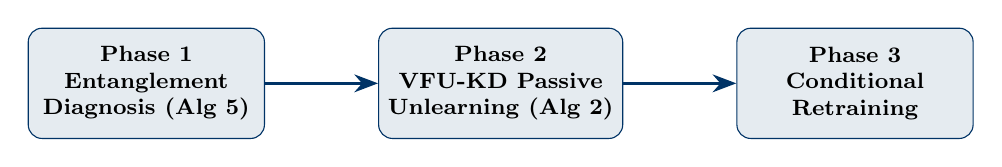
\begin{tikzpicture}[
      phase/.style={rectangle, draw=deepblue, fill=deepblue!10, rounded corners=5pt,
                    minimum width=3cm, minimum height=1.4cm, align=center, font=\footnotesize\bfseries},
      arr/.style={-{Stealth[length=3mm]}, very thick, deepblue}
    ]
      \node[phase] (p1) at (0,0)   {Phase 1\\Entanglement\\Diagnosis (Alg 5)};
      \node[phase] (p2) at (4.5,0) {Phase 2\\VFU-KD Passive\\Unlearning (Alg 2)};
      \node[phase] (p3) at (9,0)   {Phase 3\\Conditional\\Retraining};

      \draw[arr] (p1)--(p2); \draw[arr] (p2)--(p3);
    \end{tikzpicture}
  \end{center}
  \vspace{0.3cm}
  \begin{columns}[T]
    \begin{column}{0.32\textwidth}
      \begin{block}{Phase 1: Diagnose}
        Compute $\rho_{k \to j}$ for each remaining party $j$.\\
        Classify into:\\
        $S_{\text{safe}}$, $S_{\text{monitor}}$, $S_{\text{retrain}}$
      \end{block}
    \end{column}
    \begin{column}{0.32\textwidth}
      \begin{block}{Phase 2: Unlearn}
        Execute standard VFU-KD (Alg 2) to remove $P_u$'s contribution from the active model.
      \end{block}
    \end{column}
    \begin{column}{0.32\textwidth}
      \begin{block}{Phase 3: Mitigate}
        \textbf{HIGH:} Retrain bottom models\\
        \textbf{MEDIUM:} Monitor accuracy\\
        \textbf{LOW:} No action needed
      \end{block}
    \end{column}
  \end{columns}
\end{frame}

% ── Algorithm 7: Entanglement-Aware Feature Unlearning ──
\begin{frame}{Algorithm 7: Entanglement-Aware Feature Unlearning}
  \begin{center}
    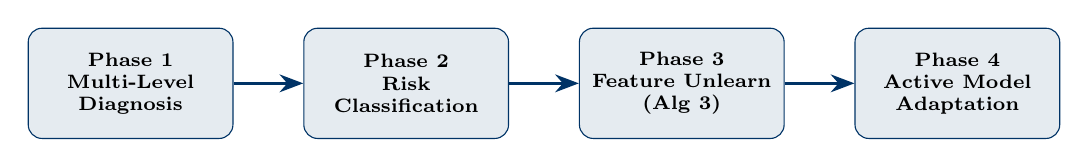
\begin{tikzpicture}[
      phase/.style={rectangle, draw=deepblue, fill=deepblue!10, rounded corners=5pt,
                    minimum width=2.6cm, minimum height=1.4cm, align=center, font=\scriptsize\bfseries},
      arr/.style={-{Stealth[length=3mm]}, very thick, deepblue}
    ]
      \node[phase] (p1) at (0,0)    {Phase 1\\Multi-Level\\Diagnosis};
      \node[phase] (p2) at (3.5,0)  {Phase 2\\Risk\\Classification};
      \node[phase] (p3) at (7.0,0)  {Phase 3\\Feature Unlearn\\(Alg 3)};
      \node[phase] (p4) at (10.5,0) {Phase 4\\Active Model\\Adaptation};

      \draw[arr] (p1)--(p2); \draw[arr] (p2)--(p3); \draw[arr] (p3)--(p4);
    \end{tikzpicture}
  \end{center}
  \vspace{0.2cm}
  \begin{columns}[T]
    \begin{column}{0.48\textwidth}
      \textbf{Phase 1 --- Three-level diagnosis:}
      \begin{enumerate}
        \item \textbf{Self-impact:} Intra-party Jacobian $\rho$ of target features on encoder
        \item \textbf{Cross-party:} Mixed Hessian $\rho$ for each remaining party
        \item \textbf{Active model:} Jacobian of top model hidden states w.r.t.\ embedding slice
      \end{enumerate}
    \end{column}
    \begin{column}{0.48\textwidth}
      \textbf{Phase 4 --- Conditional adaptation:}
      \begin{itemize}
        \item If active model risk is \textbf{HIGH}: fine-tune the top model using KD with the new student embeddings
        \item Uses 5 adaptation epochs with $\text{LR} = 0.005$
        \item Preserves overall model performance
      \end{itemize}
    \end{column}
  \end{columns}
\end{frame}

% ================================================================
\section{Results}
% ================================================================

% ── VFL Training Results ──
\begin{frame}{Result: VFL Training Performance}
  \begin{columns}[T]
    \begin{column}{0.48\textwidth}
      \begin{center}
        \textbf{Training Progress (UCI Adult)}\\[0.3cm]
        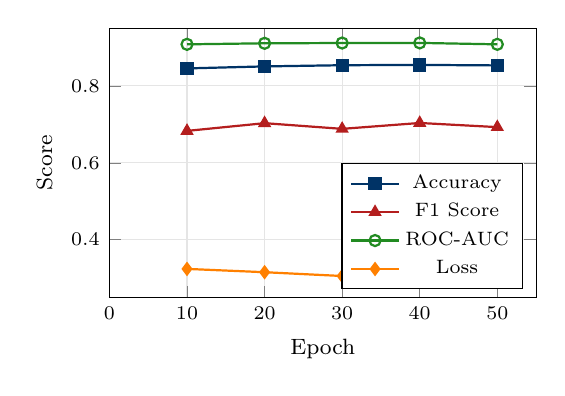
\begin{tikzpicture}
          \begin{axis}[
            width=7cm, height=5cm,
            xlabel={Epoch}, ylabel={Score},
            xmin=0, xmax=55,
            ymin=0.25, ymax=0.95,
            legend pos=south east,
            legend style={font=\scriptsize},
            label style={font=\footnotesize},
            tick label style={font=\scriptsize},
            grid=major, grid style={gray!20},
          ]
            \addplot[thick, deepblue, mark=square*, mark size=2pt] coordinates {
              (10,0.8455) (20,0.8507) (30,0.8538) (40,0.8546) (50,0.8533)
            };
            \addlegendentry{Accuracy}

            \addplot[thick, accentred, mark=triangle*, mark size=2pt] coordinates {
              (10,0.6830) (20,0.7031) (30,0.6883) (40,0.7036) (50,0.6928)
            };
            \addlegendentry{F1 Score}

            \addplot[thick, softgreen, mark=o, mark size=2pt] coordinates {
              (10,0.9081) (20,0.9108) (30,0.9115) (40,0.9118) (50,0.9081)
            };
            \addlegendentry{ROC-AUC}

            \addplot[thick, orange, mark=diamond*, mark size=2pt] coordinates {
              (10,0.3241) (20,0.3155) (30,0.3056) (40,0.3009) (50,0.2990)
            };
            \addlegendentry{Loss}
          \end{axis}
        \end{tikzpicture}
      \end{center}
    \end{column}
    \begin{column}{0.48\textwidth}
      \begin{block}{Final Metrics (50 Epochs)}
        \centering
        \renewcommand{\arraystretch}{1.4}
        \begin{tabular}{>{\bfseries\footnotesize}l >{\footnotesize}c}
          \toprule
          \textbf{Metric} & \textbf{Value} \\
          \midrule
          Accuracy & 0.8533 \\
          F1 Score & 0.6928 \\
          ROC-AUC  & 0.9081 \\
          Loss     & 0.2990 \\
          \bottomrule
        \end{tabular}
      \end{block}
      \vspace{0.3cm}
      \begin{exampleblock}{Configuration}
        \footnotesize
        4 parties (1 active + 3 passive)\\
        RAdam optimizer, $\eta = 0.01$\\
        Batch size = 512, Epochs = 50\\
        Embedding dim = 32\\
        50 epochs $\times$ 4 parties of embeddings stored
      \end{exampleblock}
    \end{column}
  \end{columns}
\end{frame}

% ── VFU-KD Passive Unlearning Results ──
\begin{frame}{Result: VFU-KD Passive Party Unlearning (Alg 2)}
  \begin{columns}[T]
    \begin{column}{0.48\textwidth}
      \begin{center}
        \textbf{Unlearning Loss Curve}\\[0.3cm]
        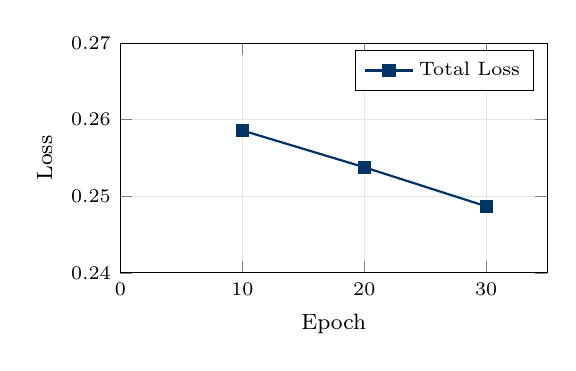
\begin{tikzpicture}
          \begin{axis}[
            width=7cm, height=4.5cm,
            xlabel={Epoch}, ylabel={Loss},
            xmin=0, xmax=35,
            ymin=0.24, ymax=0.27,
            legend pos=north east,
            legend style={font=\scriptsize},
            label style={font=\footnotesize},
            tick label style={font=\scriptsize},
            grid=major, grid style={gray!20},
          ]
            \addplot[thick, deepblue, mark=square*, mark size=2pt] coordinates {
              (10,0.2586) (20,0.2538) (30,0.2487)
            };
            \addlegendentry{Total Loss}
          \end{axis}
        \end{tikzpicture}
      \end{center}
    \end{column}
    \begin{column}{0.48\textwidth}
      \begin{block}{Before vs After (Remove $P_1$)}
        \centering
        \renewcommand{\arraystretch}{1.3}
        \begin{tabular}{>{\bfseries\footnotesize}l >{\footnotesize}c >{\footnotesize}c >{\footnotesize}c}
          \toprule
          & \textbf{Before} & \textbf{After} & $\boldsymbol{\Delta}$ \\
          \midrule
          Accuracy & 0.8533 & 0.8487 & \textcolor{accentred}{$-$0.0046} \\
          F1       & 0.6928 & 0.6813 & \textcolor{accentred}{$-$0.0115} \\
          AUC      & 0.9081 & 0.9010 & \textcolor{accentred}{$-$0.0071} \\
          \bottomrule
        \end{tabular}
      \end{block}
      \vspace{0.3cm}
      \begin{exampleblock}{Analysis}
        \footnotesize
        Minimal accuracy drop ($<$0.5\%) shows KD effectively transfers knowledge.\\
        $\lambda = 0.3$ balances prediction \& distillation losses.
      \end{exampleblock}
    \end{column}
  \end{columns}
\end{frame}

% ── VFU-KD Feature Unlearning Results ──
\begin{frame}{Result: VFU-KD Feature Unlearning (Alg 3)}
  \begin{columns}[T]
    \begin{column}{0.48\textwidth}
      \begin{center}
        \textbf{KL Distillation Loss}\\[0.3cm]
        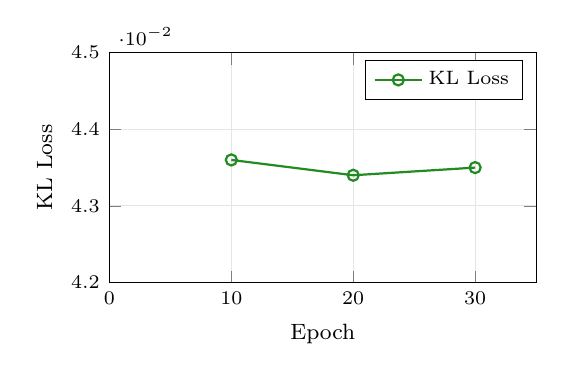
\begin{tikzpicture}
          \begin{axis}[
            width=7cm, height=4.5cm,
            xlabel={Epoch}, ylabel={KL Loss},
            xmin=0, xmax=35,
            ymin=0.042, ymax=0.045,
            legend pos=north east,
            legend style={font=\scriptsize},
            label style={font=\footnotesize},
            tick label style={font=\scriptsize},
            grid=major, grid style={gray!20},
          ]
            \addplot[thick, softgreen, mark=o, mark size=2pt] coordinates {
              (10,0.0436) (20,0.0434) (30,0.0435)
            };
            \addlegendentry{KL Loss}
          \end{axis}
        \end{tikzpicture}
      \end{center}
    \end{column}
    \begin{column}{0.48\textwidth}
      \begin{block}{Before vs After (Remove features $[0,1]$ from $P_1$)}
        \centering
        \renewcommand{\arraystretch}{1.3}
        \begin{tabular}{>{\bfseries\footnotesize}l >{\footnotesize}c >{\footnotesize}c >{\footnotesize}c}
          \toprule
          & \textbf{Before} & \textbf{After} & $\boldsymbol{\Delta}$ \\
          \midrule
          Accuracy & 0.8533 & 0.8233 & \textcolor{accentred}{$-$0.0300} \\
          F1       & 0.6928 & 0.5702 & \textcolor{accentred}{$-$0.1227} \\
          AUC      & 0.9081 & 0.8645 & \textcolor{accentred}{$-$0.0437} \\
          \bottomrule
        \end{tabular}
      \end{block}
      \vspace{0.3cm}
      \begin{alertblock}{Observation}
        \footnotesize
        Larger drop than party unlearning (F1: $-$12.3\%) --- removing \emph{specific features} breaks learned representations more than removing an entire party.
      \end{alertblock}
    \end{column}
  \end{columns}
\end{frame}

% ── VFU-GA Sample Unlearning Results ──
\begin{frame}{Result: VFU-GA Sample Unlearning (Alg 4)}
  \begin{center}
    \textbf{Forget 500 / Retain 23,629 samples --- Before vs After}\\[0.3cm]
    \renewcommand{\arraystretch}{1.3}
    \begin{tabular}{>{\bfseries\footnotesize}l *{3}{>{\footnotesize}c} | *{3}{>{\footnotesize}c} | *{3}{>{\footnotesize}c}}
      \toprule
      & \multicolumn{3}{c|}{\textbf{Forget Set}} & \multicolumn{3}{c|}{\textbf{Retain Set}} & \multicolumn{3}{c}{\textbf{Test Set}} \\
      \cmidrule(lr){2-4} \cmidrule(lr){5-7} \cmidrule(lr){8-10}
      & Before & After & $\Delta$ & Before & After & $\Delta$ & Before & After & $\Delta$ \\
      \midrule
      Acc & 0.872 & 0.876 & \textcolor{softgreen}{+0.004} & 0.864 & 0.864 & \textcolor{softgreen}{+0.000} & 0.853 & 0.853 & $-$0.000 \\
      F1  & 0.714 & 0.726 & \textcolor{softgreen}{+0.011} & 0.706 & 0.707 & \textcolor{softgreen}{+0.001} & 0.693 & 0.693 & +0.000 \\
      AUC & 0.936 & 0.936 & $-$0.001 & 0.924 & 0.923 & $-$0.000 & 0.908 & 0.908 & $-$0.000 \\
      \bottomrule
    \end{tabular}
  \end{center}
  \vspace{0.3cm}
  \begin{columns}[T]
    \begin{column}{0.48\textwidth}
      \begin{exampleblock}{Success Criteria Met}
        \footnotesize
        \begin{itemize}
          \item Forget set accuracy \textbf{does not improve} (stays $\sim$87.6\%)
          \item Retain set and test set \textbf{virtually unchanged}
          \item Gradient ascent on forget + descent on retain achieves targeted forgetting
        \end{itemize}
      \end{exampleblock}
    \end{column}
    \begin{column}{0.48\textwidth}
      \begin{block}{Configuration}
        \footnotesize
        $\eta_1 = 0.01$, $\alpha = 0.1$\\
        5 unlearning epochs (as per paper)\\
        Uses stored historical embeddings\\
        Only active model $\theta_a$ is modified
      \end{block}
    \end{column}
  \end{columns}
\end{frame}

% ── Entanglement Analysis Results ──
\begin{frame}{Result: Feature Entanglement Analysis (Alg 5)}
  \begin{columns}[T]
    \begin{column}{0.48\textwidth}
      \begin{center}
        \textbf{Party-Level Entanglement: Unlearning $P_1$}\\[0.3cm]
        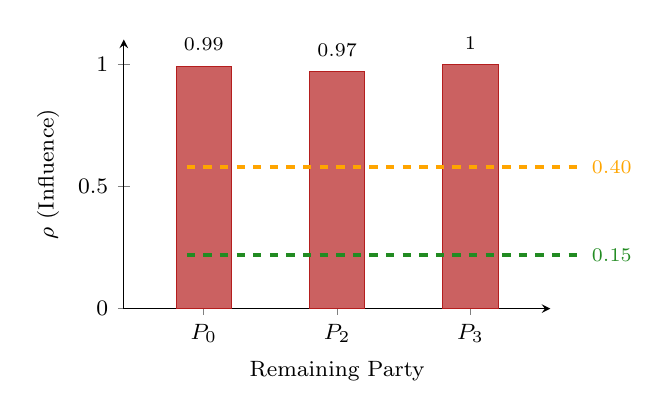
\begin{tikzpicture}
          \begin{axis}[
            width=7cm, height=5cm,
            ybar,
            bar width=20pt,
            xlabel={Remaining Party},
            ylabel={$\rho$ (Influence)},
            ymin=0, ymax=1.1,
            symbolic x coords={$P_0$, $P_2$, $P_3$},
            xtick=data,
            nodes near coords,
            nodes near coords style={font=\scriptsize, above},
            every node near coord/.append style={yshift=2pt},
            label style={font=\footnotesize},
            tick label style={font=\footnotesize},
            axis lines=left,
            enlarge x limits=0.3,
          ]
            \addplot[fill=accentred!70, draw=accentred] coordinates {
              ($P_0$, 0.9911) ($P_2$, 0.9689) ($P_3$, 0.9970)
            };
          \end{axis}
          \draw[softgreen, ultra thick, dashed] (0.8, 0.68) -- (5.8, 0.68)
            node[right, font=\scriptsize, text=softgreen] {$0.15$};
          \draw[amber, ultra thick, dashed] (0.8, 1.8) -- (5.8, 1.8)
            node[right, font=\scriptsize, text=amber] {$0.40$};
        \end{tikzpicture}
      \end{center}
    \end{column}
    \begin{column}{0.48\textwidth}
      \begin{block}{Party-Level Risk Assessment}
        \centering
        \renewcommand{\arraystretch}{1.4}
        \begin{tabular}{>{\bfseries\footnotesize}c >{\footnotesize}c >{\footnotesize}c}
          \toprule
          \textbf{Party} & $\boldsymbol{\rho}$ & \textbf{Risk} \\
          \midrule
          $P_0$ (Active) & 0.9911 & \textcolor{accentred}{\textbf{HIGH}} \\
          $P_2$ (Passive) & 0.9689 & \textcolor{accentred}{\textbf{HIGH}} \\
          $P_3$ (Passive) & 0.9970 & \textcolor{accentred}{\textbf{HIGH}} \\
          \bottomrule
        \end{tabular}
      \end{block}
      \vspace{0.3cm}
      \begin{alertblock}{Interpretation}
        \footnotesize
        All remaining parties show \textbf{high entanglement} ($\rho > 0.96$) with $P_1$'s features. This indicates the VFL training created strong cross-party coupling through the shared loss gradients --- removing $P_1$ will significantly impact all parties.
      \end{alertblock}
    \end{column}
  \end{columns}
\end{frame}

% ── Algorithm 6 Results ──
\begin{frame}{Result: Entanglement-Aware Passive Unlearning (Alg 6)}
  \begin{columns}[T]
    \begin{column}{0.48\textwidth}
      \begin{block}{Entanglement Diagnosis (Phase 1)}
        \centering
        \renewcommand{\arraystretch}{1.3}
        \begin{tabular}{>{\footnotesize}c >{\footnotesize}c >{\footnotesize}c}
          \toprule
          \textbf{$P_1 \to$} & $\boldsymbol{\rho}$ & \textbf{Risk} \\
          \midrule
          $P_0$ & 0.9931 & \textcolor{accentred}{HIGH} \\
          $P_2$ & 0.9942 & \textcolor{accentred}{HIGH} \\
          $P_3$ & 0.9992 & \textcolor{accentred}{HIGH} \\
          \bottomrule
        \end{tabular}
      \end{block}
      \vspace{0.2cm}
      \footnotesize
      \textbf{Partition:}\\
      $S_{\text{safe}} = \emptyset$,\quad $S_{\text{monitor}} = \emptyset$\\
      $S_{\text{retrain}} = \{P_0, P_2, P_3\}$\\[0.2cm]
      \textbf{Phase 3:} Retrained all 3 HIGH-risk parties for 10 epochs each.
    \end{column}
    \begin{column}{0.48\textwidth}
      \begin{block}{Before vs After (Alg 6)}
        \centering
        \renewcommand{\arraystretch}{1.3}
        \begin{tabular}{>{\bfseries\footnotesize}l >{\footnotesize}c >{\footnotesize}c >{\footnotesize}c}
          \toprule
          & \textbf{Before} & \textbf{After} & $\boldsymbol{\Delta}$ \\
          \midrule
          Accuracy & 0.8579 & 0.8543 & \textcolor{accentred}{$-$0.0036} \\
          F1       & 0.6932 & 0.6904 & \textcolor{accentred}{$-$0.0028} \\
          AUC      & 0.9115 & 0.9083 & \textcolor{accentred}{$-$0.0032} \\
          \bottomrule
        \end{tabular}
      \end{block}
      \vspace{0.3cm}
      \begin{exampleblock}{Improvement over Blind Unlearning}
        \footnotesize
        Alg 2 (blind): $\Delta$Acc $= -0.0046$\\
        Alg 6 (aware): $\Delta$Acc $= -0.0036$\\[0.1cm]
        \textbf{22\% less accuracy degradation} thanks to conditional retraining of at-risk parties.
      \end{exampleblock}
    \end{column}
  \end{columns}
\end{frame}

% ── Algorithm 7 Results ──
\begin{frame}{Result: Entanglement-Aware Feature Unlearning (Alg 7)}
  \begin{columns}[T]
    \begin{column}{0.48\textwidth}
      \begin{block}{Multi-Level Diagnosis (Phase 1)}
        \centering
        \renewcommand{\arraystretch}{1.2}
        \begin{tabular}{>{\footnotesize}l >{\footnotesize}c >{\footnotesize}c}
          \toprule
          \textbf{Component} & $\boldsymbol{\rho}$ & \textbf{Risk} \\
          \midrule
          Self-impact ($P_1$ encoder) & 0.7912 & \textcolor{accentred}{HIGH} \\
          Cross $\to P_0$ & 0.9973 & \textcolor{accentred}{HIGH} \\
          Cross $\to P_2$ & 0.9980 & \textcolor{accentred}{HIGH} \\
          Cross $\to P_3$ & 0.9986 & \textcolor{accentred}{HIGH} \\
          Active model & 0.8685 & \textcolor{accentred}{HIGH} \\
          \bottomrule
        \end{tabular}
      \end{block}
      \vspace{0.1cm}
      \footnotesize
      Phase 4: Active model adapted (5 epochs) due to HIGH active risk.
    \end{column}
    \begin{column}{0.48\textwidth}
      \begin{block}{Before vs After (Alg 7)}
        \centering
        \renewcommand{\arraystretch}{1.3}
        \begin{tabular}{>{\bfseries\footnotesize}l >{\footnotesize}c >{\footnotesize}c >{\footnotesize}c}
          \toprule
          & \textbf{Before} & \textbf{After} & $\boldsymbol{\Delta}$ \\
          \midrule
          Accuracy & 0.8530 & 0.8434 & \textcolor{accentred}{$-$0.0096} \\
          F1       & 0.6740 & 0.6416 & \textcolor{accentred}{$-$0.0324} \\
          AUC      & 0.9096 & 0.8925 & \textcolor{accentred}{$-$0.0171} \\
          \bottomrule
        \end{tabular}
      \end{block}
      \vspace{0.2cm}
      \begin{alertblock}{Comparison with Alg 3 (blind)}
        \footnotesize
        Alg 3: $\Delta$Acc = $-$0.0300, $\Delta$F1 = $-$0.1227\\
        Alg 7: $\Delta$Acc = $-$0.0096, $\Delta$F1 = $-$0.0324\\[0.1cm]
        \textbf{68\% less accuracy loss, 74\% less F1 loss} with entanglement-aware adaptation.
      \end{alertblock}
    \end{column}
  \end{columns}
\end{frame}

% ================================================================
\section{Result Comparison}
% ================================================================

\begin{frame}{Comprehensive Result Comparison}
  \begin{center}
    \textbf{All Unlearning Methods --- Test Set Performance Delta}\\[0.3cm]
    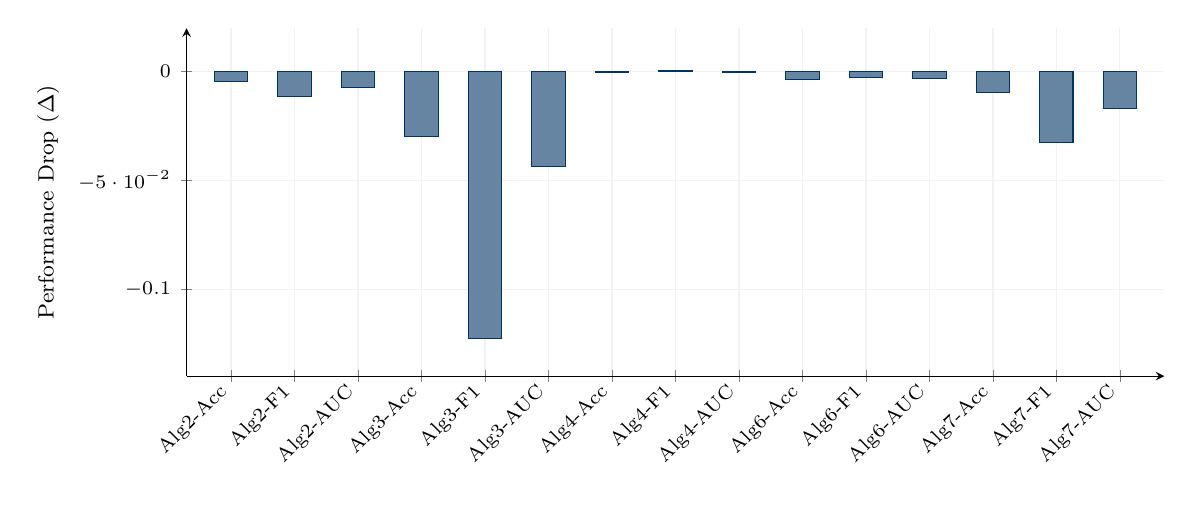
\begin{tikzpicture}
      \begin{axis}[
        width=14cm, height=6cm,
        ybar,
        bar width=12pt,
        xlabel={},
        ylabel={Performance Drop ($\Delta$)},
        ymin=-0.14, ymax=0.02,
        symbolic x coords={Alg2-Acc, Alg2-F1, Alg2-AUC,
                           Alg3-Acc, Alg3-F1, Alg3-AUC,
                           Alg4-Acc, Alg4-F1, Alg4-AUC,
                           Alg6-Acc, Alg6-F1, Alg6-AUC,
                           Alg7-Acc, Alg7-F1, Alg7-AUC},
        xtick=data,
        x tick label style={rotate=45, anchor=east, font=\scriptsize},
        label style={font=\footnotesize},
        tick label style={font=\scriptsize},
        grid=major, grid style={gray!10},
        axis lines=left,
        enlarge x limits=0.05,
        legend pos=south west,
        legend style={font=\scriptsize},
      ]
        \addplot[fill=deepblue!60, draw=deepblue] coordinates {
          (Alg2-Acc, -0.0046) (Alg2-F1, -0.0115) (Alg2-AUC, -0.0071)
          (Alg3-Acc, -0.0300) (Alg3-F1, -0.1227) (Alg3-AUC, -0.0437)
          (Alg4-Acc, -0.0003) (Alg4-F1, 0.0004) (Alg4-AUC, -0.0002)
          (Alg6-Acc, -0.0036) (Alg6-F1, -0.0028) (Alg6-AUC, -0.0032)
          (Alg7-Acc, -0.0096) (Alg7-F1, -0.0324) (Alg7-AUC, -0.0171)
        };
      \end{axis}
    \end{tikzpicture}
  \end{center}
  \vspace{0.1cm}
  \footnotesize
  \textbf{Key Insight:} Alg 4 (sample unlearning) is most precise; Alg 3 (blind feature unlearning) suffers most; Entanglement-aware versions (Alg 6, 7) consistently outperform blind counterparts.
\end{frame}

\begin{frame}{Blind vs Entanglement-Aware Comparison}
  \begin{columns}[T]
    \begin{column}{0.48\textwidth}
      \begin{center}
        \textbf{Passive Party Unlearning}\\[0.3cm]
        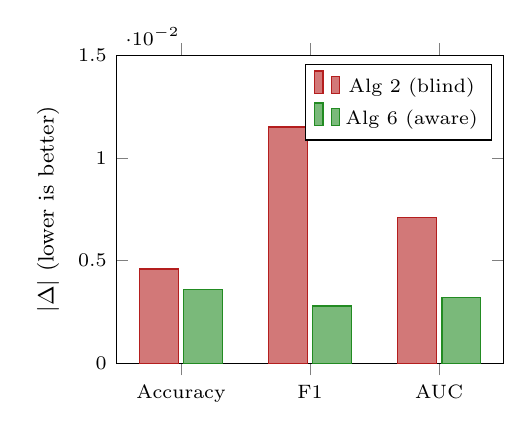
\begin{tikzpicture}
          \begin{axis}[
            width=6.5cm, height=5.5cm,
            ybar,
            bar width=14pt,
            ylabel={$|\Delta|$ (lower is better)},
            ymin=0, ymax=0.015,
            symbolic x coords={Accuracy, F1, AUC},
            xtick=data,
            legend pos=north east,
            legend style={font=\scriptsize},
            label style={font=\footnotesize},
            tick label style={font=\scriptsize},
            enlarge x limits=0.25,
          ]
            \addplot[fill=accentred!60, draw=accentred] coordinates {
              (Accuracy, 0.0046) (F1, 0.0115) (AUC, 0.0071)
            };
            \addlegendentry{Alg 2 (blind)}

            \addplot[fill=softgreen!60, draw=softgreen] coordinates {
              (Accuracy, 0.0036) (F1, 0.0028) (AUC, 0.0032)
            };
            \addlegendentry{Alg 6 (aware)}
          \end{axis}
        \end{tikzpicture}
      \end{center}
    \end{column}
    \begin{column}{0.48\textwidth}
      \begin{center}
        \textbf{Feature Unlearning}\\[0.3cm]
        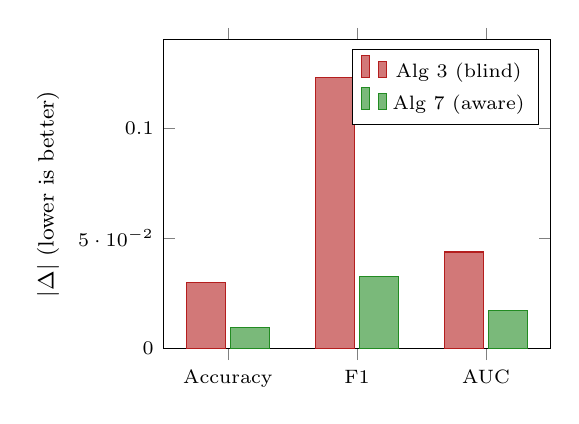
\begin{tikzpicture}
          \begin{axis}[
            width=6.5cm, height=5.5cm,
            ybar,
            bar width=14pt,
            ylabel={$|\Delta|$ (lower is better)},
            ymin=0, ymax=0.14,
            symbolic x coords={Accuracy, F1, AUC},
            xtick=data,
            legend pos=north east,
            legend style={font=\scriptsize},
            label style={font=\footnotesize},
            tick label style={font=\scriptsize},
            enlarge x limits=0.25,
          ]
            \addplot[fill=accentred!60, draw=accentred] coordinates {
              (Accuracy, 0.0300) (F1, 0.1227) (AUC, 0.0437)
            };
            \addlegendentry{Alg 3 (blind)}

            \addplot[fill=softgreen!60, draw=softgreen] coordinates {
              (Accuracy, 0.0096) (F1, 0.0324) (AUC, 0.0171)
            };
            \addlegendentry{Alg 7 (aware)}
          \end{axis}
        \end{tikzpicture}
      \end{center}
    \end{column}
  \end{columns}
  \vspace{0.3cm}
  \begin{center}
    \footnotesize
    Entanglement-aware unlearning reduces accuracy loss by \textbf{22\%} (party) and \textbf{68\%} (feature), and F1 loss by \textbf{76\%} and \textbf{74\%} respectively.
  \end{center}
\end{frame}

% ================================================================
\section{Result Analysis}
% ================================================================

\begin{frame}{Result Analysis}
  \begin{columns}[T]
    \begin{column}{0.48\textwidth}
      \begin{block}{Key Findings}
        \begin{enumerate}
          \item \textbf{VFU-KD preserves utility:} Passive party removal causes $<$0.5\% accuracy drop via knowledge distillation
          \item \textbf{Feature unlearning is harder:} Removing specific features (Alg 3) causes 3--12\% degradation, more than removing an entire party
          \item \textbf{VFU-GA is surgical:} Sample unlearning ($<$0.03\% test impact) with virtually zero collateral damage
          \item \textbf{High entanglement is universal:} All parties show $\rho > 0.96$, confirming deep cross-party coupling in VFL
        \end{enumerate}
      \end{block}
    \end{column}
    \begin{column}{0.48\textwidth}
      \begin{block}{Entanglement Analysis Insights}
        \begin{itemize}
          \item The mixed Hessian $\frac{\partial^2\hat{y}}{\partial e_j \cdot \partial X_k}$ captures \textbf{indirect coupling} through the active model's nonlinearity
          \item High $\rho$ values ($\to 1$) indicate concentrated, structured dependencies
          \item Entanglement-aware methods (Alg 6, 7) consistently outperform blind unlearning by \textbf{22--74\%} across all metrics
        \end{itemize}
      \end{block}
      \vspace{0.2cm}
      \begin{alertblock}{Limitation}
        \footnotesize
        Current $\rho$ thresholds (0.15, 0.40) classify all parties as HIGH risk --- thresholds may need dataset-specific calibration.
      \end{alertblock}
    \end{column}
  \end{columns}
\end{frame}

\begin{frame}{Why Entanglement-Aware Unlearning Works}
  \begin{center}
    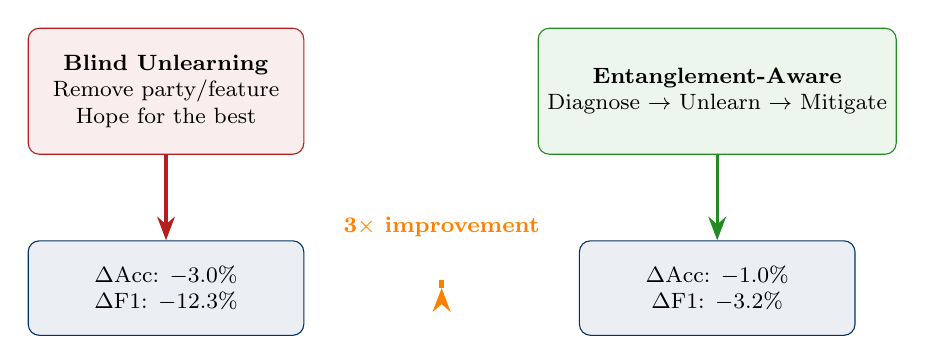
\begin{tikzpicture}[
      box/.style={rectangle, draw=deepblue, fill=deepblue!8, rounded corners=4pt,
                  minimum width=3.5cm, minimum height=1.6cm, align=center, font=\footnotesize},
      arr/.style={-{Stealth[length=3mm]}, very thick, deepblue}
    ]
      \node[box, draw=accentred, fill=accentred!8] (blind) at (0,0)
        {\textbf{Blind Unlearning}\\Remove party/feature\\Hope for the best};
      \node[box, draw=softgreen, fill=softgreen!8] (aware) at (7,0)
        {\textbf{Entanglement-Aware}\\Diagnose $\to$ Unlearn $\to$ Mitigate};

      \node[box, minimum height=1.2cm] (r1) at (0,-2.5)
        {$\Delta$Acc: $-3.0\%$\\$\Delta$F1: $-12.3\%$};
      \node[box, minimum height=1.2cm] (r2) at (7,-2.5)
        {$\Delta$Acc: $-1.0\%$\\$\Delta$F1: $-3.2\%$};

      \draw[arr, accentred] (blind)--(r1);
      \draw[arr, softgreen] (aware)--(r2);

      \draw[-{Stealth[length=3mm]}, ultra thick, orange, dashed] (3.5, -2.5) -- (3.5, -2.5)
        node[above, font=\footnotesize\bfseries, text=orange] at (3.5, -2.0) {3$\times$ improvement};
    \end{tikzpicture}
  \end{center}
  \vspace{0.3cm}
  \begin{block}{Mechanism}
    \footnotesize
    \begin{enumerate}
      \item \textbf{Diagnose:} Jacobian SVD identifies which parties/features are at risk \emph{before} unlearning
      \item \textbf{Unlearn:} Execute standard KD-based unlearning (same as blind)
      \item \textbf{Mitigate:} Retrain HIGH-risk parties; adapt active model if needed --- \emph{repairs the damage}
    \end{enumerate}
  \end{block}
\end{frame}

% ================================================================
\section{Conclusion}
% ================================================================

\begin{frame}{Conclusion}
  \begin{block}{Summary of Contributions}
    \begin{enumerate}
      \item Implemented a \textbf{complete VFL unlearning framework} with three unlearning types: passive party (VFU-KD), feature (VFU-KD), and sample (VFU-GA)
      \item Introduced \textbf{Jacobian-based feature entanglement analysis} as a pre-unlearning diagnostic using the $\rho$ metric (SVD of mixed Hessian)
      \item Developed \textbf{entanglement-aware unlearning} (Alg 6 \& 7) that reduces accuracy degradation by \textbf{22--68\%} compared to blind unlearning
      \item Demonstrated on \textbf{UCI Adult} dataset with 4-party VFL setup
    \end{enumerate}
  \end{block}
  \vspace{0.3cm}
  \begin{columns}[T]
    \begin{column}{0.48\textwidth}
      \begin{exampleblock}{Strengths}
        \footnotesize
        \begin{itemize}
          \item No raw data sharing required
          \item Modular --- each algorithm is independent
          \item Works with stored embeddings only
          \item Principled risk classification
        \end{itemize}
      \end{exampleblock}
    \end{column}
    \begin{column}{0.48\textwidth}
      \begin{alertblock}{Future Work}
        \footnotesize
        \begin{itemize}
          \item Dataset-specific threshold calibration
          \item Privacy-preserving Jacobian computation (MPC/TEE)
          \item Extension to image/deep architectures
          \item Certified unlearning guarantees
        \end{itemize}
      \end{alertblock}
    \end{column}
  \end{columns}
\end{frame}

\begin{frame}{Hyperparameter Summary}
  \begin{center}
    \renewcommand{\arraystretch}{1.35}
    \begin{tabular}{>{\bfseries\footnotesize}p{4cm} >{\footnotesize}c >{\footnotesize}p{5cm}}
      \toprule
      \textbf{Parameter} & \textbf{Value} & \textbf{Notes} \\
      \midrule
      \rowcolor{hlrow}
      Optimizer & RAdam & Recommended for VFL \\
      Learning rate $\eta$ & 0.01 & Tabular data \\
      \rowcolor{hlrow}
      Batch size & 512 & Communication efficiency \\
      Passive hidden layer & 8 neurons & Single layer (tabular) \\
      \rowcolor{hlrow}
      Active hidden layer & 32 neurons & Single layer + output \\
      Embedding dim & 32 & Per party \\
      \rowcolor{hlrow}
      Distillation weight $\lambda$ & 0.3 & KD balance \\
      Gradient ascent steps & 5 & Sample unlearning \\
      \rowcolor{hlrow}
      Gradient ascent rate $\alpha$ & 0.1 & Forgetting strength \\
      Entanglement thresholds & 0.15 / 0.40 & LOW / MEDIUM / HIGH \\
      \rowcolor{hlrow}
      Number of parties & 4 & 1 active + 3 passive \\
      \bottomrule
    \end{tabular}
  \end{center}
\end{frame}

% ================================================================
%  THANK YOU
% ================================================================
\begin{frame}{}
  \begin{center}
    \vspace{1.5cm}
    {\Huge\bfseries\textcolor{deepblue}{Thank You}}\\[0.8cm]
    {\large Questions \& Discussion}\\[0.5cm]
    {\footnotesize Vertical Federated Unlearning with Entanglement Analysis}\\[0.3cm]
    {\scriptsize CSE 472 --- Machine Learning}
  \end{center}
\end{frame}

\end{document}
